% \documentclass{report}

% \usepackage{fancyhdr}
\usepackage{fourier-orns}
\usepackage{hyperref}%% To refrence links / jumps
\usepackage{chngcntr} %% For some extra counters numberings
\usepackage[a4paper, right = 0.5in, left = 0.5in,top = 1in , bottom = 1in]{geometry}
\usepackage{etoolbox} %% Provides like a language for advanced customization
\usepackage{datetime} %% For dates of course
\usepackage{lastpage} %% provides pages numbers
\usepackage[sc]{titlesec} %% modify titles
\usepackage{enumerate}
\usepackage{cancel}
\usepackage{tikzsymbols}
\usepackage[dvipsnames]{xcolor}
\usepackage{import}
\usepackage{pdfpages} %% include other pdfs
\usepackage{transparent} %% Transparency
\usepackage{xcolor}  %% Colors
\usepackage[many]{tcolorbox}
\usepackage[framemethod=TikZ]{mdframed}
\usepackage{amsmath,amsfonts,amsthm,amssymb,mathtools}
\usepackage{tikz}
\usepackage{bookmark}
\usepackage{graphicx}
\usepackage{mathpazo}

\usepackage{fontawesome5}

\linespread{1.5}


\titleformat{\chapter}[display]   
{\fontfamily{ppl}\selectfont\huge\color{YellowOrange!80!orange}} % Font style and size 
{\raggedleft\color{purple}\fontsize{70}{0pt}\selectfont\thechapter}   
{-1.5cm}    			                          % Space between the chapter number and title
{
	\begin{tikzpicture}[overlay]
		\node[anchor = west,yshift = 0.2cm,xshift = -1cm] {\fontsize{90}{20} $\int_{}^{} $};
		\node[yshift = 4cm, xshift = 17cm]   {\includegraphics[width = 4cm]{preview0}};
	\end{tikzpicture}
\hspace{1cm}\Huge\raggedright\MakeUppercase}

\titleformat{\section}[block]
{
\fontfamily{ppl}\selectfont\huge\color{YellowOrange!80!orange}
}
{
\color{purple}\fontsize{20}{0pt}\selectfont\thesection 
}
{0cm}
{
	\begin{tikzpicture}[overlay]
		\node[anchor = west,yshift = 0.2cm,xshift = -0.4cm, circle = 1pt] {};
	\end{tikzpicture}
}

\titlespacing*{\section}{0pt}{0.7cm}{1.5cm}


\newcommand{\divider}
{
	\begin{center}
	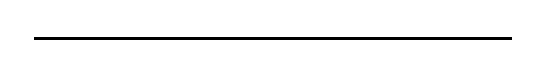
\begin{tikzpicture}
		\draw[thick, black] (0.25*\textwidth, 0) -- (0.75*\textwidth, 0);
		\node[rotate = 360 - 90, xshift = -0.6pt, yshift = 1pt] at (0.25*\textwidth,0){\decotwo};
		\node[rotate = 90, xshift = -0.6pt, yshift = 1pt] at (0.75*\textwidth,0){\decotwo};
	\end{tikzpicture}
	\end{center}
}

\pagestyle{fancy}

\newcommand{\lecday}[1][]
{
    \def\datee{#1}
    \fancyhead[L]{\datee}
}



\newcommand{\signature}
{
	\begin{tikzpicture}[remember picture,overlay]
		\node[fill = YellowOrange!20!white] at ([yshift = 1cm, xshift = -3cm]current page.south east) {\fontsize{10pt}{0pt}{\itshape Kara.$\mathcal{A}$}};
	\end{tikzpicture}
}

\AddToHook{shipout/background}{
  \begin{tikzpicture}[remember picture, overlay]
	  \node[] at ([yshift = 1.5cm,xshift = \textwidth /2 + 0.9cm]current page.south west) {\includegraphics[width = 0.5cm]{preview3}};
	  \node[] at ([yshift = 1.5cm,xshift = - \textwidth /2 - 0.9cm]current page.south east) {\includegraphics[width = 0.5cm]{preview4}};
  \end{tikzpicture}
}



\newtcolorbox[auto counter, number within = section]{remark}[1][]
{
       		title = Remark #1,
		enhanced,
		boxrule = 0pt,
		colback = white,
		breakable,
		arc = 4pt,
		colbacktitle = cyan,
		colback = cyan!5!white,
		segmentation style =
		{
			solid,cyan,thick,
		},
		attach boxed title to top left =
		{
			xshift = 0cm,
		},
		boxed title style =
		{
			boxrule = 0pt,
			sharp corners,
			drop fuzzy shadow = {cyan},
		},
		drop fuzzy shadow = {cyan!80!black},
}

\newtcolorbox[auto counter, number within = section]{theorem}[1][]
{                                      
		title = Theorem \thetcbcounter : #1,
		enhanced, 
		boxrule = 0pt,
		colback = white,
		breakable,
		arc = 4pt,
		colbacktitle = purple,
		colback = purple!5!white,
		segmentation style = 
		{
			solid, purple,thick,
		},
		attach boxed title to top left = 
		{
			xshift = 0cm, 
		},
		boxed title style = 
		{
			boxrule = 0pt,
			sharp corners,
			drop fuzzy shadow = {purple},
		},
		drop fuzzy shadow = {purple!80!black},
}

\newtcolorbox[auto counter, number within = section]{definition}[1][]
{                                      
		title = Definition \thetcbcounter : #1,
		enhanced, 
		boxrule = 0pt,
		colback = white,
		arc = 4pt,
		breakable,
		colbacktitle = YellowOrange!80!black,
		segmentation style = 
		{
			solid, YellowOrange,thick,
		},
		attach boxed title to top left = 
		{
			xshift = 0cm, 
		},
		colback = YellowOrange!5!white,
		boxed title style = 
		{
			boxrule = 0pt,
			sharp corners,
			drop fuzzy shadow = {YellowOrange!80!orange},
		},
		drop fuzzy shadow = {YellowOrange!80!black},
}

\newtcolorbox[auto counter, number within = section]{corollary}[1][]
{                                      
		title = corollary \thetcbcounter : #1,
		enhanced, 
		boxrule = 0pt,
		colback = white,
		arc = 4pt,
		breakable,
		colbacktitle = YellowOrange!80!black,
		segmentation style = 
		{
			solid, YellowOrange,thick,
		},
		attach boxed title to top left = 
		{
			xshift = 0cm, 
		},
		colback = YellowOrange!5!white,
		boxed title style = 
		{
			boxrule = 0pt,
			sharp corners,
			drop fuzzy shadow = {YellowOrange!80!orange},
		},
		drop fuzzy shadow = {YellowOrange!80!black},
}


\newtcolorbox{example}[1][]
{                                      
		title = Example,
		enhanced, 
		boxrule = 0pt,
		colback = white,
		arc = 4pt,
		segmentation style = 
		{
			solid, SpringGreen,thick,
		},
		breakable,
		colback = SpringGreen!5!white,
		colbacktitle = SpringGreen!80!black,
		attach boxed title to top left = 
		{
			xshift = 0cm, 
		},
		boxed title style = 
		{
			boxrule = 0pt,
			sharp corners,
			drop fuzzy shadow = {SpringGreen!80!orange},
		},
		drop fuzzy shadow = {SpringGreen!80!black},
}


\newcommand{\integral}[4]{\int\limits_{#1}^{#2} #4 d#3}
\newcommand{\limit}[3]{\lim\limits_{#1 \rightarrow #2} #3}
\newcommand{\strone}[2]{\left[ \begin{gathered}#1\\ #2\end{gathered} \right] }
\newcommand{\strtwo}[2]{\left\{ \begin{gathered}#1\\ #2\end{gathered} \right\} }
\newcommand{\strthree}[2]{\left\lfloor \begin{gathered}#1\\ #2\end{gathered} \right\rfloor }


\newcommand{\startbf}[1]{\text{\bfseries{#1}}}
\newcommand{\sett}[1]{\left\{ #1 \right\}}
\newcommand{\thesis}[1]{\left( #1 \right)}
\newcommand{\brkt}[1]{\left[ #1 \right]}
\newcommand{\floor}[1]{\left\lfloor #1 \right\rfloor}


\DeclareMathOperator{\img}{im} % Image
\DeclareMathOperator{\Img}{Im} % Image
\DeclareMathOperator{\coker}{coker} % Cokernel
\DeclareMathOperator{\Coker}{Coker} % Cokernel
\DeclareMathOperator{\Ker}{Ker} % Kernel
\DeclareMathOperator{\rank}{rank}
\DeclareMathOperator{\Spec}{Spec} % spectrum
\DeclareMathOperator{\Tr}{Tr} % trace
\DeclareMathOperator{\pr}{pr} % projection
\DeclareMathOperator{\ext}{ext} % extension
\DeclareMathOperator{\pred}{pred} % predecessor
\DeclareMathOperator{\dom}{dom} % domain
\DeclareMathOperator{\ran}{ran} % range
\DeclareMathOperator{\Hom}{Hom} % homomorphism
\DeclareMathOperator{\Mor}{Mor} % morphisms
\DeclareMathOperator{\End}{End} % endomorphism


\newcommand{\lm}{\ensuremath{\lambda}}
\newcommand{\eps}{\ensuremath{\epsilon}}
\newcommand{\veps}{\ensuremath{\varepsilon}}
\newcommand{\al}{\ensuremath{\alpha}}
\newcommand{\bb}{\ensuremath{\beta}}
\newcommand{\cc}{\ensuremath{\gamma}}
\newcommand{\dd}{\ensuremath{\delta}}
\newcommand{\DD}{\ensuremath{\Delta}}
\newcommand{\ff}{\ensuremath{\phi}}
\newcommand{\FF}{\ensuremath{\varphi}}

\newcommand{\RR}{\mathbb{R}}
\newcommand{\RO}{\mathcal{R}}
\newcommand{\EE}{\mathbb{E}}
\newcommand{\CC}{\mathbb{C}}
\newcommand{\RW}{\mathbb{R}^2}
\newcommand{\RT}{\mathbb{R}^3}
\newcommand{\RN}{\mathbb{R}^n}
\newcommand{\DS}{\mathcal{D}}

\newcommand{\KK}{\mathbb{K}}
\newcommand{\KW}{\mathbb{K}^2}
\newcommand{\KT}{\mathbb{K}^3}
\newcommand{\KN}{\mathbb{K}^n}

\newcommand{\NN}{\mathbb{N}}

\newcommand{\PS}{\mathcal{P}}
\newcommand{\AS}{\mathcal{E}}
\newcommand{\FS}{\mathcal{F}}
\newcommand{\LS}{\mathcal{L}}
\newcommand{\MS}{\mathcal{M}}


















\lecday[2025-02-06]

% \begin{document}
\large


\section{Examples of norms on 
	\texorpdfstring{$\RN$}{Rn} and 
	\texorpdfstring{$\CC^n$}{Cn}}
\begin{example}
	\begin{enumerate}
	\item In $\RR $ (Considered as $\RR $ vector space), the usual
		norm is the absolute value, in $\CC $ (Considered
		as $\CC $ vector space), the usual norm is the modulus.
	\item  Let $n \geq 2$ be an integer, we may define 
		on $\KN$ (Considered as $\KK$ vector space), several norms
		including. 
		$\left\{ \|  \| _{1}, \|  \| _{2}, \|  \| _{p} \right\}$, with 
		$\left( p \geq 1 \right)$, and $\|  \| _{\infty }$, the norms
		we just stated are the most widely used, they are defined by : 
		\begin{align*}
			\| x \| _{1} &:= 
			\sum_{i=1}^{n} \left| x_{i} \right|
			\\
			\| x \| _{2} &:=
			\sqrt{ \sum_{i=1}^{n} \left| 
			x_{i}\right|^2  }  = 
			\left( \sum_{i=1}^{n} \left| x_{i} \right|^2  \right)^{
			\frac{1}{2}}
			\\
			\| x \| _{p} &:=
			\left( 
				\sum_{i=1}^{n}  \left| x_{i} \right|^{p}
			\right)^{\frac{1}{p}} \\
			\| x \| _{\infty } &:= 
			\max_{1 \leq i \leq n} \left| x_{i} \right|
		\end{align*}
		Both in $\RN$  and in $\CC ^{n}$  $\left( n \in \NN \right)$, 
		the norm $\| .\| _{2}$  is called
		the euclidean norm, and the norm
		$\|  .\| _{p}$  $\left( p \geq 1 \right)$  is called
		the Holder norm of exponent $p$ (or simpley, the $p$-norm).\\
		Remark that $\|.  \| _{1}$  and $\|.  \| _{2}$ are special
		cases of $\|.  \| _{p}$. We can also show that :
		\[
		\lim_{n \to \infty} \| . \| _{p} = 
		\| . \| _{\infty }
		\]
		Further, it's easy to show that the norms 
		\[
		\| . \| _{p} \quad \forall p \geq 1 \text{ are equivallent } 
		\]
		Prove that $\| . \| _{1} \sim \| . \| _{\infty }$ and 
		$\| . \| _{2} \sim \| . \| _{1}$. (Hint : $n 
		\left( 
			( \max \left| x_{i} \right| )^2 
		\right)^{1/2}
	       $)
	\end{enumerate}
	Furthermore, its easy to show
	that the norms
	$\| . \| _{p} \left( p \geq 1 \right)$, 
	are all equivalent (they are even equal 
	for $n=1$), To show that 
	$\| . \| _{p} \left( p \geq 1 \text{ 
	arbitrary } \right)$, is really a norm
	on $\KN$, only the triangle inequality
	that poses a problem, (The special 
	cases $p=1$, and $p = \infty $ are
	easy), we fix this problem by solving the following 
	exercise below !
\end{example}
\begin{center}
	\textbf{
Consider the following exercise : 
	}
\end{center}
Let $n$ be a positive integer and let $p,q > 1$, such that 
$\frac{1}{p} + \frac{1}{q} = 1$. 
\begin{enumerate}[(i)]
	\item By using the connexity of the exponential function,
		show that for all positive real numbers $a$ and $b$, we have
		\[
		a \cdot  b \leq 
		\frac{a ^{p}}{p} + 
		\frac{b^{q}}{q}
		\]
		(Known as The Young Inequality)
	\item Deduce that for all positive real numbers 
		$x_1,x_2, ..., x_{n}, y_1, y_2, \hdots , y_{n}$, we have :
		\[
		\sum_{i=1}^{n} x_{i} y_{i} 
		\leq 
		\left( 
			\sum_{i=1}^{n} x_{i}^{p}
		\right)^{1/p}  
		+
		\left( 
			\sum_{i=1}^{n} 
			y_{i}^{p}
		\right)^{1/p}
		\] 
		(Known as the Holder Inequality) 
\item 
	Deduce that for all positive
	real numbers $x_1,x_2, ...
	, x_{n}, y_1,y_2, ..., y_{n}$, we have : 
	\[
		\left( 
	\sum_{i=1}^{n} 
	\left( x_{i}+y_{i} \right)^{p}
		\right)^{1/p} \leq 
		\left( 
			\sum_{i=1}^{n} 
			x_{i}^{p}
		\right)^{1/p} + 
		\left( 
			\sum_{i=1}^{n} 
			y_{i}^{p}
		\right)^{1/p}
	\]
	(Called the Minkowski Inequality)
\item Conclude that $\| . \| $  is really
	a norm on $\KK^{n}$  where 
	$\left( K = \RR \text{ or } \CC \right)$ 
\end{enumerate}
\begin{center}
	\textbf{Solution : }
\end{center}
\begin{enumerate}[(i)]
	\item 
		Since the function 
		$u \rightarrow e^{u}$  is 
		convex on $\RR $ because
		$\left( (e^{u})^{''} = 
		e^{u} > 0\right)$, then 
		we have for all  
		$t \in [0,1]$  and for all
		$x,y \in \RR $  :
		\[
			e^{tx + \left( 1-t \right)y} \leq 
			te^{x}  + 
			\left( 1-t \right)e^{y}
		\]
		We apply the above for 
		$t = \frac{1}{p}$  so 
		$\left( 1-t \right) = 1 - 
		\frac{1}{p} = \frac{1}{q}$, and for 
		$x,y$ such that 
		$e^{x} = a ^{p}$ (i.e. 
		$x = p \ln{\left( a \right)}$ ), and 
		$e^{y} = b ^{q}$  (i.e. 
		$y = q \ln{\left( b \right)}$ ) we obtain
		that : 
		\begin{align*}
		\left( a ^{p} \right)^{1/p} 
		\left( b ^{q} \right)^{1/q} 
		&\leq  
		\frac{a ^{p}}{p} + 
		\frac{b^{q}}{q} \\
			a \cdot b & \leq 
		\frac{a ^{p}}{p} + 
		\frac{b^{q}}{q} 
		\end{align*}
		as required.
	\item Let 
		$x_1,x_2, ..., x_{n}, 
		y_1,y_2, ..., y_{n} >  0$,
		for $i \in \left\{ 
			1,2, \hdots , n
		\right\}$, by applying 
		the Young inequality 
		proved above for 
		$a = \frac{x_{i}}{
		(\sum_{i=1}^{n} x_{j}^{p})^{1/p}}$ 
		and $b = 
		\frac{y_{i}}{
			\left( 
				\sum_{j=1}^{n} 
				y_{j}^{q}
			\right)^{1/q}
		}
		$
		we get : 
	\[
	\frac{x_{i}y_{i}}{
		\left( 
			\sum_{j = 1}^{n}  
			x_{j}^{p}
		\right)^{1/p}
		\left( 
			\sum_{j=1}^{n} 
			y_{j}^{q}
		\right)^{1/q} 
	}                      
	\leq 
		\frac{1}{p}
		\left[ 
		\frac{x_{i}^{p}}{
		\sum_{j=1}^{n} 
	x_{j}^{p}} 
		\right]
		+ 
		\frac{1}{q}
		\left[ 
			\frac{y_{i}^{q}}{
				\sum_{j=1}^{n} 
				y_{j}^{q}
			}
		\right]
	\]
	Next, by taking the summation from 
	$i=1$ to $n$, in the two sides of his last inequality
	, we get : 
	\begin{align*}
	\frac{\sum_{i=1}^{n} 
x_{i}y_{i}}{
\left( 
	\sum_{j=1}^{n} 
	x_{j}^{p}
\right)^{1/p} 
\left( 
	\sum_{j=1}^{n} 
	y_{j}^{q}
\right)^{1/q}
}
&\leq 
\frac{1}{p} + 
\frac{1}{q} = 1 \\
\sum_{i=1}^{n} 
       x_{i}y_{i} & \leq 
       \left( 
	       \sum_{i=1}^{n} 
	       x_{i}^{p}
       \right)^{1/p} 
       \left( 
	       \sum_{j=1}^{n} 
	       y_{j}^{q}
       \right)^{1/q}
	\end{align*}
	As required\\
	Remark that the Holder inequality
generalizes, the Cauchy-Schawrtz Inequality for 
the usual inner product of $\RN$ (take $p=q=2$).
\item Let $x_1,x_2, ..., x_{n}, y_1,y_2, ..., y_{n}>0$,
	we have : 
	\begin{align*}
	\sum_{i=1}^{n} 
	\left( x_{i} + y_{i} \right)^{p} 
	&= 
	\sum_{i=1}^{n}  
	\left( x_{i} + y_{i} \right)
	\left( x_{i} + y_{i} \right) ^{p-1} \\
	&= 
	\sum_{i=1}^{n} 
	x_{i} \left( 
	x_{i} + y_{i}\right)^{p-1} +
	\sum_{i=1}^{n} 
	y_{i} \left( 
		x_{i} + y_{i}
	\right)^{p-1}
	\end{align*}
	Then by applying the Holder inequality,
	for each of the two sums 
	$\sum_{i=1}^{n} 
	x_{i}\left( x_{i}+ y_{i} \right)^{p-1}$  
	and 
	$\sum_{i=1}^{n} y_{i}
	\left( x_{i} + y_{i} \right)^{p-1}$  we derive
	that : 
	\[
	\sum_{i=1}^{n} 
	\left( x_{i} + y_{i} \right)^{p} \leq 
	\left( 
		\sum_{i=1}^{n} 
		x_{i}^{p}
	\right)^{1/p} 
	\left( 
		\sum_{i=1}^{n}  
		\left( x_{i} + y_{i} \right) 
		^{\left( p-1 \right)q} 
	\right)^{1/q} + 
	\left( 
		\sum_{i=1}^{n} 
		y_{i}^{p}
	\right)^{1/p} 
	\left( 
		\sum_{i=1}^{n} 
		\left( x_{i}+y_{i} \right) 
		^{\left( p-1 \right)q}
	\right)^{1/q}
	\]
	And since $\left( p-1 \right)q = p$  
	(Because $\frac{1}{p} + \frac{1}{q} = 
	1$), it follows that : 
	\begin{align*}
	\sum_{i=1}^{n} 
	\left( x_{i} + y_{i} \right)^{p} 
	& \leq 
	\left( 
		\sum_{i=1}^{n} 
		\left( x_{i} + y_{i} \right)
		^{p}
	\right)^{1/q} 
	\left(
	\left( 
		\sum_{i=1}^{n} 
		x_{i}^{p}
	\right)^{1/p}
	+ 
	\left( 
		\sum_{i=1}^{n} 
		y_{i}^{p}
	\right)^{1/p}
	\right)
	\\
	\left( 
		\sum_{i=1}^{n} 
		\left( x_{i} + y_{i} \right)^{p}
	\right)^{1 - \frac{1}{q}} & 
	\leq 
	\left( 
		\sum_{i=1}^{n} 
		x_{i}^{p}
	\right)^{1/p} + 
	\left( \sum_{i=1}^{n} 
	y_{i}^{p}\right)^{1/p} \\
		\left( 
			\sum_{i=1}^{n} 
			\left( 
			x_{i} + y_{i}\right) 
			^{p}
		\right)^{1/p} 
				  &\leq 
		\left( 
			\sum_{i=1}^{n} 
			x_{i}^{p}
		\right)^{1/p} + 
		\left( 
			\sum_{i=1}^{n} 
			y_{i}^{p}
		\right)^{1/p}
	\end{align*}
\item The two first properties of a norm
	$\left( \text{ i.e. }, (i) 
	\text{ and }  (ii)) \right)$, are clearly
	satisfied by $\| . \| _{p}$ , so it remains 
	to shows the triangle
	inequality 
	$\left( \| x+y \| _{p} \leq 
	\| x \|_{p} + \| y \| _{p} \quad 
\forall  x,y \in \KK^{n}\right)$. First, remark 
that the Minkowski Inequality (proved above), 
remains true for 
$x_1,x_2, ..., x_{n}, y_1,y_2, ..., y_{n} > 0$ (That is if
some if the $x_{i}$'s and 
$y_{i}$'s are zero), This can be justified
by the continuity for example now, for 
\[
X := 
\begin{pmatrix}
	x_1 \\
	x_2 \\
	\vdots  \\
	x_{n} \\
\end{pmatrix}
\quad 
Y := 
\begin{pmatrix}
	y_1 \\
	y_2 \\
	\vdots  \\
	y_{n} \\
\end{pmatrix}
\in \KK^{n}
\]
We have that : 
\begin{align*}
\| x+y \| _{p} = 
\left( \sum_{i=1}^{n} 
	\| x_{i} + y_{i} \| ^{p}
\right)^{1/p} \leq 
\left( 
	\sum_{i=1}^{n} 
	\underbrace{
	\left( 
		\left| x_{i} \right| +
		\left| y_{i} \right|
	\right)^{p}
}_{\in  [0,\infty)} 
\right)^{1/p}
\leq 
\left( 
	\sum_{i=1}^{n} 
	\left| x_{i} \right|^{p}
\right)^{1/p} + 
\left( 
	\sum_{i=1}^{n} 
	\left| y_{i} \right|^{p}
\right)^{1/p} 
\end{align*}
According to the Minkowsky Inequality we get
it equal 
\begin{align*}
\left( 
	\sum_{i=1}^{n} 
	\left| x_{i} \right|^{p}
\right)^{1/p} + 
\left( 
	\sum_{i=1}^{n} 
	\left| y_{i} \right|^{p}
\right)^{1/p}  = 
\| x \| _{p} + 
\| y \| _{p}
\end{align*}
As required, Consequently, 
$\| . \| _{p}$  is a norm on $\CC ^{n}$ 
\end{enumerate}
\section{Finite product of normed vector spaces}
Let $\left( E_1,N_1 \right),
\left( E_2,N_2 \right), \hdots , \left( E_{k},N_{k} \right)
\quad  \left( k \geq 1 \right)$, be normed
vector spaces over $\KK= \RR \text{ or } \CC $, and 
set $E := E_1 \times E_2 \times \hdots \times E_{k}$. \\
We may define on $E$ several norms which are expressed in 
terms of $N_1,N_2, \hdots , N_{k}$. Among these norms
we set :
\begin{itemize}
	\item $\| . \|_{1}: 
		\quad \forall x = 
		\begin{pmatrix}
			x_1 \\
			x_2 \\
			\vdots  \\
			x_{k} \\
		\end{pmatrix}
		\in E : \quad 
		\| x \| _{1} :=
		\sum_{i=1}^{k} 
		N_{i}\left( x_{i} \right)
		$ 
	\item 
		$
	        \| . \| _{2}: \quad 
		\forall x = 
		\begin{pmatrix}
			x_1 \\
			x_2 \\
			\vdots  \\
			x_{k} \\
		\end{pmatrix} 
		\in E: \quad 
		\| x \| _{2} :=
		\left( 
			\sum_{i=1}^{k} 
			N_{i}\left( x_{i} \right)^2 
		\right)^{1/2}
		$ 
	\item 
		$
		\| . \| _{p}: \quad 
		\forall x = 
		\begin{pmatrix}
			x_1 \\
			x_2 \\
			\vdots  \\
			x_{k} \\
		\end{pmatrix} 
		\in E: \quad 
		\| x \| _{p} :=
		\left(              
			\sum_{i=1}^{k} 
			N_{i}\left( x_{i} \right)^p 
		\right)^{1/p}
		$ 
	\item 
		$
		\| . \| _{\infty }: \quad 
		\forall x = 
		\begin{pmatrix}
			x_1 \\
			x_2 \\
			\vdots  \\
			x_{k} \\
		\end{pmatrix} 
		\in E: \quad 
		\| x \| _{\infty } :=
		\max _{1 \leq i \leq k}
		N_{i}\left( x_{i} \right)
		$ 
\end{itemize}
We can show that all the norms 
$\| . \| _{p} \quad \left( 
	1 \leq p \leq \infty 
\right)$ are equivalent, and that the common toplogy
generated by them is the product topology
of $E$. This allows us to affirm that, A toplogical
product of a finite number of N.V.S is a N.V.S.
%"Produit denombrable d'une espace normé est né pas
%forcément un espace normé"
\\
Note that this last result is in general false
for a toplogical product of an infinite number
of normed vector spaces.
\section{Exampels of norms of an infinite-dimensional
vector space}
Let $a,b \in \RR $ with $a < b$, The $\RR-$vector space
\[
E := \mathcal{C} ^{a}
\left( 
	[a,b] , \RR 
\right) \quad 
\text{ Contituted of continiuous functions on $[a,b] $ } 
\]
Can be equipped with several importants norms, including
$\| . \| _{1}, 
\| . \| _{2}, \| . \| _{p} \quad 
\left( p \geq 1 \right)$  and 
$\| . \| _{\infty }$ 
% \end{document}
